\chapter{Problemanalyse}\label{ch:problemanalyse}

\section{Sværme}
% I dette afsnit skal der udvælges en sværm, baseret på 
% Overordnet definition og vores definition for resten af rapporten
%Skal der noget med sværmintelligens med her?



%En sværm er ifølge \cite{definition} en \textit{"større gruppe af mindre dyr, oftest insekter eller fugle, der tæt samlet bevæger sig af sted"}, når der i nærværende projekt tales om sværme, er det ud fra denne definition. 

\subsection{Typer af sværme}
% Eksempler på typer af sværme og organismer indenfor hver type

\subsection{Valg af sværm}
% Konklusion på forrige afsnit. Hvilken sværm vælger vi? Og hvorfor?



\section{Metoder til oversættelse af bevægelser}
I dette afsnit, vil det blive undersøgt nærmere, hvilke metoder der findes til at oversætte bevægelser i naturen, til modeller og software en computer kan forstå. 
% Start 
% Hvilke muligheder er der for at oversætte bevægelserne? (Regel-baseret, boids, maskinlæring)

\subsection{Regel-baseret}
% Forklaring af regel-baserede systemer
Et regel-baseret system er en type af kunstig intelligens, der behandler information baseret på et antal regler, der på forhånd er defineret af mennesker. Et sådan system er i stand til at efterligne en ekspert på området. En eksperts viden er repræsenteret af systemets regler, samt en række fakta om det relevante systems begyndelsestilstand. Disse regler er ofte af formen "if-then", hvilket betyder at en resulterende konklusion eller handling, kun vil finde sted hvis betingelsen er opfyldt \cite{Grosan2011}. Disse systemer kræver derfor at der er opstillet klart definerede regler til at dække alle handlinger der kan foretages inden for systemets arbejdsområde.\\
Regel-baserede systemer kan anvendes inden for flere områder, såsom klassifikation, eksempelvis diagnose af sygdom baseret på symptomer, og forudsigelser af konsekvenserne af ændringer i et system. 
\par
% Eksempel med boids på regel-baseret model. 
Der findes også regel-baserede modeller, som er modeller defineret indirekte ud fra nogle regler. Et eksempel på en sådan regel-baseret model, er boid modellen fra \cite{boids}. Denne bruges til at modellere de enkelte elementer i en simuleret flok. Denne model er baseret på tre regler: kollisionsundgåelse, hastighedsmatching og flokcentrering. Ud fra disse regler dannes en model for de enkelte medlemmer i en flok, der gør dem i stand til at danne, og vedligeholde en flok.
\par
% Forklarer at der er tale om top-dowm i regelbaseret.
Sådanne regel-baserede systemer og modeller er en såkaldt top-down fremgangsmåde. Hvilket betyder at de regler systemerne bygger på, bliver lavet på baggrund af undersøgelser af den type subjekt det ønskes at modellere.
\par
% Lille eksempel med modellering af fisks bevægelser
Et eksempel på dette er \cite{RAILSBACK199973}, hvor der laves en række regler om hvordan fisk bevæger sig. Dette gøres baseret på en gennemgang af litteratur der undersøger og modellerer netop dette. Resultaterne sammenlignes herefter med observationer af hvordan sådanne fisk egentlig bevæger sig, og der gøres forsøg på at lave regler der stemmer mere overens med den observerede adfærd.
\par
Top-down fremgangsmåden fremstår i, at de enkelte aspekter der har indflydelse på subjektets beslutninger og overordnede opførsel modelleres, baseres på analyse af den generelle adfærd. 
% Forklarer hvorfor vi ikke vil have top-down
\par
Dette er ikke en hensigtsmæssig tilgang, i situationer hvor det ønskes at lave en model, men de nødvendige regler ikke er kendt på forhånd. I sådanne tilfælde er det nødvendigt at udarbejde regler for samtlige aspekter af subjektets adfærd. Ydermere er der et behov for at verificere at disse regler afspejler denne adfærd korrekt.

\subsection{Maskinlæring}
Maskinlæring er en metode til at få en computer til at finde mønstre i data, uden at programmøren skal specificere præcist hvordan det skal gøres [CITATION]. Det afviger fra traditionel programmering, ved at man overlader selve udformningen af løsningen af en given opgave til computeren, og i stedet giver den et mål den skal sigte efter [CITATION]. Det er oftest optimeringsopgaver der bliver overladt til maskinlæring, men disse optimeringsopgaver kan variere drastisk i deres anvendelsesområder. Maskinlæring er blevet brugt til at lave musik \cite{mlmusic}, optimere ..., designe ...

\\\\
Weak ai
general purpose ai
\\\\
\textbf{Deep learning}\\
Deep learning er inspireret af hjernen som har neuroner. Deep learning tager et bestemt element ind og prøver kører inutet igennem forskellige lag. Her har deep learning en masse værktøjer i lagene som bruges til at opnå et resultat. Man kender ikke til hvad der sker i lagene som ikke er indput og outpu 
\\\\
%https://towardsdatascience.com/supervised-unsupervised-and-deep-learning-aa61a0e5471c
\textbf{Supervised maskinlæring}\\
Ved supervised maskinlæring lærer maskinen ud fra mærket træningsdata hvor dataen allerede er blevet kategoriseret. Denne træningsdata indeholder elementer som har nogle variabler på træk som kendetegner en kategori. Maskinen generer, ud fra træningsdataen, en model for træk som er typisk for en bestemt kategori. På den måde kan maskinen forsøge at kategorisere nye elementer ud fra dens træk ved at sammenligne elementets variabler med hvad maskinen allerede har lært.
\\\\
Denne type for maskinlæring er blevet brugt indenfor...
\\\\
\textbf{Unsupervised}\\
Unsupervised maskinlæring går ud på at maskinen får det samme input som en supervised, dog uden en kategori. I stedet for placere input i kategorier, så smider den dem ind i en model efter variablerne. Alt input som ønskes at blive kategoriseret har typisk træk i form af varibler og dette betyder at input i samme kategori har det med at ligge ved siden i modelen. I modellen er en klynge af input derfor en kategori som har meget tilfælles.
\\\\
Denne type for maskinlæring er blevet brugt indenfor...
\\\\
\textbf{Reinforcement læring}\\
Reinforcementlæring handler om at maskinen får tildelt et element og prøver derefter kategorisere elementet. Hvis elementets kategori allerede er kendt, kan maskinen få fortalt om maskinen har gættet rigtigt eller forkert. Den prøver derefter at ændre sin model, så der er større sandsynlighed for at gætte rigtigt næste gang.
\\\\
Denne type for maskinlæring er blevet brugt indenfor...

Ai programmeringsprog tensorflow, python
\subsection{Mini-konklusion}
% Valg af maskinlæring og hvorfor
Der er ikke en præcis model for hvordan denne type af sværm bevæger sig, og derfor vil der være en udfordring at tage en regel-baseret tilgang. Det giver derimod god mening at bruge en form for maskinlæring til at finde denne model, da denne metode er i stand til at modellere adfærd uden sådanne regler.


\section{Maskinlæring}
% hvad er maskinlæring?
% Introduktion til afsnittet

Neural networking
Learning algorithms.


% Kun så specifikt som vi er i stand til inden problemløsningen
% Hvordan fungerer de og hvad bruges de til?

\subsection{Læring}

\subsubsection*{Supervised}
Overvåget, superviseret
\\\\
Supervised learning, eller overvåget læring, er en træningsfunktion der bliver givet et datasæt, hvori de rigtige resultater er markeret, så funktionen ved hvilket resultat den skal frem til. Dette kan sammenlignes med hvis et menneske skulle gennemgå nogle data og finde frem til nogle resultater, at de havde en supervisor som kender svarene og kan hjælpe dem med om de er på vej den rigtige vej\citep{Jeanmonod2018}.
\par
% Kort forklaring af backpropagation - hører nok under et afsnit om neurale netværk.
Backpropagation er en metode der bruges til at udregne gradienten i et feed-forward neuralt netværk. Denne gradient beskriver hvordan vægtene i det neurale netværk skal justeres, for at resultatet bevæger sig mod et minimum af cost-funktionen. 
\par
Et neuralt netværk trænes ved at give den træningseksempler, hvor det ønskede svar allerede er kendt. Derfor er det muligt at afgøre hvor stor fejlen er i det sidste lag i netværket, ved at sammenligne netværkets resultat med det korrekte resultat. Herefter propageres der baglæns i netværket, ved at udregne fejlen i et lag, ud fra fejlen i det efterfølgende lag\cite{Nielsen2015}. Resultatet af denne backpropogation er som sagt en gradient der angiver hvordan vægte og bias i de enkelte lag skal justeres, for at optimere cost-funktionen, og dermed resultatet. 
\\\\
Her bliver træningsfunktionen givet et datasæt med mærkater. Den ved altså hvad der hænger sammen med hvad.
\\\\



\subsubsection*{Unsupervised}
\\\\
Her bliver træningsfunktionen givet input, der ikke er markeret med det rigtige output, og computeren må så prøve sig frem. Handler mere om at gå på opdagelse, undersøge de mekanismer der opstår. Denne type læring er god til at finde ligheder i store datasæt \cite{Jeanmonod2018}.
\\\\
\newpage
\textbf{Association learning}\\ 
Association learning kan bruges til markedsanalyse, katalog design, den er generelt finde mønstre i data. Et eksempel på brug af dette kunne være en butik. I dette eksempel har vi variabler der dækker over alle butikkens varer, og en Xj  værdi, som bliver påført én af to værdier, enten 1 hvis en af disse varer bliver købt, f.eks. varer y, og 0 hvis den ikke gør. Her lære algoritmen så hvilke ting der bliver købt sammen, og kan dermed være til stor hjælp til f.eks. markedsanalyse eller design af et katalog\cite{Rodriguez-Perez1994}.
\\\\
\textbf{Cluster analyse}\\
Cluster analyser har flere forskellige mål. Alle disse mål er relaterede til gruppering eller segmentering af objekter i disse ”clusters”. Disse objekter bliver sorteret således at objekter i det samme cluster har mere til fælles end objekter fra forskellige clustre har. Generelt er målet for en cluster analyse er graden af lighed (eller ulighed) mellem de individuelle objekter. 
Et eksempel på en cluster analyse kunne være forskelligt farvede prikker der skulle deles op i 3 "clusters"  som set på figur \ref{ClusterEksempel} nedenfor

\begin{figure}[H]
    \centering
    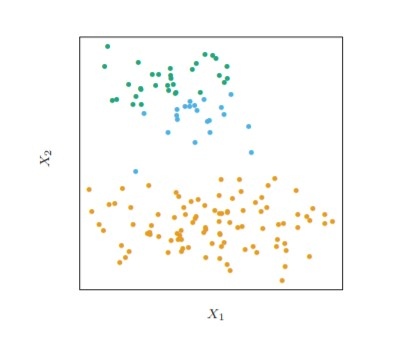
\includegraphics[width=0.7\textwidth]{figures/Cluster.jpg}
    \caption{Her ses et eksempel på en cluster analyse, hvor forskelligt farvede prikker deles op i 3 clusters \cite{Rodriguez-Perez1994}}
    \label{ClusterEksempel}
\end{figure}

Denne opdeling sker ved hjælp af en algoritme kaldet \textit{the k-means algorithm}, 


\subsubsection*{Reinforcement}
Ved denne type af læring, starter modellen typisk med en ren tavle \citep{deep-reinforcement-learning}. Modellen får ingen data med markerede svar, som i supervised læring, og må derfor prøve sig frem. En vigtig del af reinforcement læring, er at modellen får feedback på de handlinger den foretager. Dette sker igennem en fitness funktion, som belønner modellen alt efter hvor tæt på målet den er. Dette kunne være hvor hurtigt modellen kan finde vej, fra ét punkt til et andet, eller hvor tæt den er på at gætte en tekststreng eller hvor langt en simuleret bil har kørt. Fitness funktionen beregner derefter en fitness værdi ud fra hvor godt modellen klarede sig, og ud fra denne feedback, kan modellen justere sig selv, og prøve igen, indtil den kommer i mål. Der findes utallige applikationer for denne type maskinlæring, dog skal der være et klart mål med modellen, noget programmøren gerne vil optimere, da modellen skal bruge en fitness funktion \citep{deep-reinforcement-learning}. 
\par
Som tidligere nævnt, er AlphaGo et eksempel på reinforcement læring. AlphaGo har undergået flere opgraderinger, og den nyeste version, AlphaGo Zero, har lært at spille Go uden menneskelig interaktion og uden at kende noget til spillet i forvejen \citep{alphago}. Den har spillet mod sig selv igen og igen, og hver gang fået feedback på hvor godt den har klaret sig, som den så har brugt til at justere sit neurale netværk. På den måde bliver modellen bedre til at forudsige de næste træk den skal foretage, og på 40 dage blev AlphaGo Zero verdenmester i Go.
\\\\
En underkategori af reinforcement læring, er genetiske algoritmer [CITATION], som er en del af evolutions algorimter. Disse algoritmer bruger principper fra evolutionsteori, såsom selektion, reproduktion, overkrydsning, mutation og nedarvning, ud over principperne for reinforcement læring [CITATION?]. Der dannes først en befolkning af et bestemt antal agenter (mulige løsninger), som består af kromosomer. Disse kromosomer beskriver blandt andet de handler den agent kan foretage. Dette kunne eksempelvis være accelerer, drej, stop, osv.  De beskriver også andre egenskaber ved agenten, såsom hvor meget de kan se, hvor hurtigt de kan accelerere og stoppe, hvor store de er, osv. 
\par
Befolkningen af agenter køres igennem fitness funktionen, som derefter giver hver agent en fitness værdi. Herefter kommer selektionen ind i spil, og udvælgelsen kan gøres på flere forskellige måder. En af måderne det kan gøres på, er at tildele hver agent en sandsynlighed for at blive udvalgt til at reproducere, baseret på deres fitness værdi. Altså vil de agenter der har klaret sig bedst, have en større chance for at få lov til at reproducere.
\par
De agenter der udvælges til reproduktion (forældrene), bliver sat sammen, og det er her overkrydsningen sker. Dette kan også gøres på forskellige måder, men alt efter hvordan kromosomerne er indkodet, er der forskellige muligheder. Hvis kromosomerne eksempelvis er indkodet som binære strenge, kunne et punkt på kromosomet vælges, og den øverste del af den ene forældres kromosom og splejse den sammen med den nederste del af den anden forældres kromosom. Det er også her mutationen finder sted. Her kan programmøren definere en sandsynlighed for at i stedet for at tage en del af forældrenes kromosom, bliver en eller flere af værdierne hos barnets kromosom tilfældigt defineret. Dette sørger for at befolkningen hele tiden forbliver varieret, så det er muligt for modellen at udvikle den bedste løsning. Ud af dette kommer et barn, der har arvet egenskaber, igennem et kromosom der er sammensat af to eller flere forældres kromosomer. Dette barn erstatter en agent i befolkningen, så befolkningsantallet holdes konstant. Denne proces gøres så hele befolkningen er børn, og der er dermed lavet en ny generation. Denne generation bliver så kørt igennem de samme mekanismer som deres forældre, og det bliver ved indtil fitness værdien bliver høj nok, og målet er nået.
\par
Hvis variationen i befolkningen bliver for lav, kan modellen komme til at sidde fast, i den forstand at den ikke kan sammensætte forældre der er forskellige nok, til at få et nyt barn ud. Dette kan betyde at modellen plateauer langt før den kunne have gjort, hvis variationen havde været højere. Som sagt kan mutation hjælpe på at holde variationen høj, men mutationsraten må heller ikke være for høj.  En forhøjet mutationsrate kan sætte hastigheden for læringen ned, og i værste tilfælde forsage at hele modellen bare handler tilfældigt, og ikke gør sig nogen erfaringer, da alle kromosomer vil være helt tilfældige ved overkrydsning, og nedarvningen stopper [CITATION]. 
\par
En anden måde at afhjælpe en for lav variation i befolkningen, kunne være at gøre befolkningen større fra starten. Dette ville betyde at mutationerne ville ske oftere, og der ville være større sandsynlighed for at generere en god løsning hurtigere. Befolkningen må dog ikke blive for stor, da det kan nedsætte hastigheden af simulationen. Det vil sige at med en høj befolkning, kan det være at modellen kunne finde en god løsning i halvt så mange generationer som ved en lavere befolkningen, men hvis hver generation tager dobbelt så lang tid at simulere end en lavere befolkning, har man ikke vundet noget.
\\\\
Med disse mekanismer, vil kun de "stærkeste" overleve, altså dem med den højeste fitness værdi. 


\subsection{Valg af maskinlærings-metode}
% Valg af specifik metode, og hvorfor





















































% Det er her vi samles